\documentclass{standalone}
\usepackage{tikz}
\usetikzlibrary{patterns, positioning}


\begin{document}
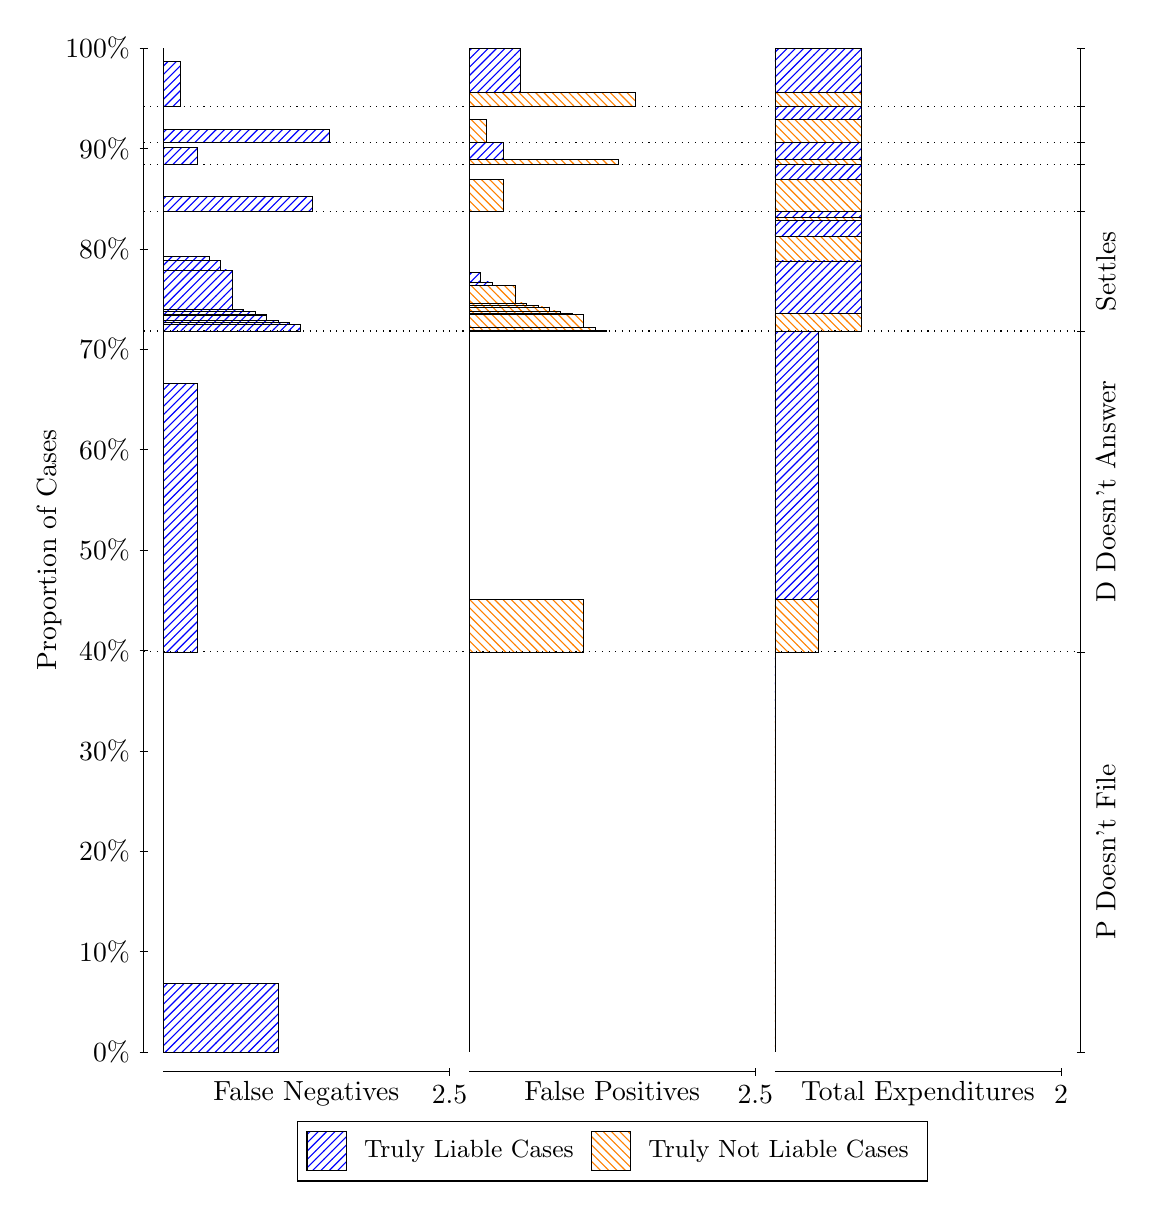
\begin{tikzpicture}
\draw[black, very thin] (1.5,1.75) -- (1.5,14.5);
\node[rotate=90, text=black, anchor=center] at (0.3, 8.125) {Proportion of Cases};
\draw[black, very thin] (1.45,1.75) -- (1.55,1.75);
\node[text=black, anchor=east] at (1.45, 1.75) {0\%};
\draw[black, very thin] (1.45,3.025) -- (1.55,3.025);
\node[text=black, anchor=east] at (1.45, 3.025) {10\%};
\draw[black, very thin] (1.45,4.3) -- (1.55,4.3);
\node[text=black, anchor=east] at (1.45, 4.3) {20\%};
\draw[black, very thin] (1.45,5.575) -- (1.55,5.575);
\node[text=black, anchor=east] at (1.45, 5.575) {30\%};
\draw[black, very thin] (1.45,6.85) -- (1.55,6.85);
\node[text=black, anchor=east] at (1.45, 6.85) {40\%};
\draw[black, very thin] (1.45,8.125) -- (1.55,8.125);
\node[text=black, anchor=east] at (1.45, 8.125) {50\%};
\draw[black, very thin] (1.45,9.4) -- (1.55,9.4);
\node[text=black, anchor=east] at (1.45, 9.4) {60\%};
\draw[black, very thin] (1.45,10.675) -- (1.55,10.675);
\node[text=black, anchor=east] at (1.45, 10.675) {70\%};
\draw[black, very thin] (1.45,11.95) -- (1.55,11.95);
\node[text=black, anchor=east] at (1.45, 11.95) {80\%};
\draw[black, very thin] (1.45,13.225) -- (1.55,13.225);
\node[text=black, anchor=east] at (1.45, 13.225) {90\%};
\draw[black, very thin] (1.45,14.5) -- (1.55,14.5);
\node[text=black, anchor=east] at (1.45, 14.5) {100\%};

\draw[black, very thin] (13.4,1.75) -- (13.4,14.5);
\draw[black, very thin] (13.35,1.75) -- (13.45,1.75);
\node[anchor=west] at (13.35, 1.75) {};
\draw[black, very thin] (13.35,6.8304) -- (13.45,6.8304);
\node[anchor=west] at (13.35, 6.8304) {};
\draw[black, very thin] (13.35,10.906) -- (13.45,10.906);
\node[anchor=west] at (13.35, 10.906) {};
\draw[black, very thin] (13.35,12.426) -- (13.45,12.426);
\node[anchor=west] at (13.35, 12.426) {};
\draw[black, very thin] (13.35,13.022) -- (13.45,13.022);
\node[anchor=west] at (13.35, 13.022) {};
\draw[black, very thin] (13.35,13.298) -- (13.45,13.298);
\node[anchor=west] at (13.35, 13.298) {};
\draw[black, very thin] (13.35,13.76) -- (13.45,13.76);
\node[anchor=west] at (13.35, 13.76) {};
\draw[black, very thin] (13.35,14.5) -- (13.45,14.5);
\node[anchor=west] at (13.35, 14.5) {};

\draw[black, very thin, pattern color=blue, pattern=north east lines] (1.75,1.75) rectangle (3.2033,2.6245);
\draw[black, very thin, pattern color=orange, pattern=north west lines] (1.75,2.6245) rectangle (1.75,6.8304);
\draw[black, very thin, pattern color=blue, pattern=north east lines] (1.75,6.8304) rectangle (2.186,10.238);
\draw[black, very thin, pattern color=orange, pattern=north west lines] (1.75,10.238) rectangle (1.75,10.906);
\draw[black, very thin, pattern color=blue, pattern=north east lines] (1.75,10.906) rectangle (3.494,10.993);
\draw[black, very thin, pattern color=blue, pattern=north east lines] (1.75,10.993) rectangle (3.3487,11.018);
\draw[black, very thin, pattern color=blue, pattern=north east lines] (1.75,11.018) rectangle (3.2033,11.043);
\draw[black, very thin, pattern color=blue, pattern=north east lines] (1.75,11.043) rectangle (3.058,11.108);
\draw[black, very thin, pattern color=blue, pattern=north east lines] (1.75,11.108) rectangle (3.058,11.113);
\draw[black, very thin, pattern color=blue, pattern=north east lines] (1.75,11.113) rectangle (2.9127,11.155);
\draw[black, very thin, pattern color=blue, pattern=north east lines] (1.75,11.155) rectangle (2.7673,11.181);
\draw[black, very thin, pattern color=blue, pattern=north east lines] (1.75,11.181) rectangle (2.622,11.681);
\draw[black, very thin, pattern color=blue, pattern=north east lines] (1.75,11.681) rectangle (2.4767,11.803);
\draw[black, very thin, pattern color=blue, pattern=north east lines] (1.75,11.803) rectangle (2.3313,11.851);
\draw[black, very thin, pattern color=orange, pattern=north west lines] (1.75,11.851) rectangle (1.75,12.426);
\draw[black, very thin, pattern color=blue, pattern=north east lines] (1.75,12.426) rectangle (3.6393,12.618);
\draw[black, very thin, pattern color=orange, pattern=north west lines] (1.75,12.618) rectangle (1.75,13.022);
\draw[black, very thin, pattern color=blue, pattern=north east lines] (1.75,13.022) rectangle (2.186,13.239);
\draw[black, very thin, pattern color=orange, pattern=north west lines] (1.75,13.239) rectangle (1.75,13.298);
\draw[black, very thin, pattern color=blue, pattern=north east lines] (1.75,13.298) rectangle (3.8573,13.468);
\draw[black, very thin, pattern color=orange, pattern=north west lines] (1.75,13.468) rectangle (1.75,13.76);
\draw[black, very thin, pattern color=blue, pattern=north east lines] (1.75,13.76) rectangle (1.968,14.328);
\draw[black, very thin, pattern color=orange, pattern=north west lines] (1.75,14.328) rectangle (1.75,14.5);
\draw[black, very thin, pattern color=orange, pattern=north west lines] (5.6333,1.75) rectangle (5.6333,5.9559);
\draw[black, very thin, pattern color=blue, pattern=north east lines] (5.6333,5.9559) rectangle (5.6333,6.8304);
\draw[black, very thin, pattern color=orange, pattern=north west lines] (5.6333,6.8304) rectangle (7.0867,7.4985);
\draw[black, very thin, pattern color=blue, pattern=north east lines] (5.6333,7.4985) rectangle (5.6333,10.906);
\draw[black, very thin, pattern color=orange, pattern=north west lines] (5.6333,10.906) rectangle (7.3773,10.918);
\draw[black, very thin, pattern color=orange, pattern=north west lines] (5.6333,10.918) rectangle (7.232,10.956);
\draw[black, very thin, pattern color=orange, pattern=north west lines] (5.6333,10.956) rectangle (7.0867,11.114);
\draw[black, very thin, pattern color=orange, pattern=north west lines] (5.6333,11.114) rectangle (6.9413,11.132);
\draw[black, very thin, pattern color=orange, pattern=north west lines] (5.6333,11.132) rectangle (6.796,11.162);
\draw[black, very thin, pattern color=orange, pattern=north west lines] (5.6333,11.162) rectangle (6.6507,11.212);
\draw[black, very thin, pattern color=orange, pattern=north west lines] (5.6333,11.212) rectangle (6.5053,11.234);
\draw[black, very thin, pattern color=orange, pattern=north west lines] (5.6333,11.234) rectangle (6.36,11.264);
\draw[black, very thin, pattern color=orange, pattern=north west lines] (5.6333,11.264) rectangle (6.2147,11.481);
\draw[black, very thin, pattern color=blue, pattern=north east lines] (5.6333,11.481) rectangle (5.924,11.529);
\draw[black, very thin, pattern color=blue, pattern=north east lines] (5.6333,11.529) rectangle (5.7787,11.651);
\draw[black, very thin, pattern color=blue, pattern=north east lines] (5.6333,11.651) rectangle (5.6333,12.426);
\draw[black, very thin, pattern color=orange, pattern=north west lines] (5.6333,12.426) rectangle (6.0693,12.83);
\draw[black, very thin, pattern color=blue, pattern=north east lines] (5.6333,12.83) rectangle (5.6333,13.022);
\draw[black, very thin, pattern color=orange, pattern=north west lines] (5.6333,13.022) rectangle (7.5227,13.081);
\draw[black, very thin, pattern color=blue, pattern=north east lines] (5.6333,13.081) rectangle (6.0693,13.298);
\draw[black, very thin, pattern color=orange, pattern=north west lines] (5.6333,13.298) rectangle (5.8513,13.589);
\draw[black, very thin, pattern color=blue, pattern=north east lines] (5.6333,13.589) rectangle (5.6333,13.76);
\draw[black, very thin, pattern color=orange, pattern=north west lines] (5.6333,13.76) rectangle (7.7407,13.932);
\draw[black, very thin, pattern color=blue, pattern=north east lines] (5.6333,13.932) rectangle (6.2873,14.5);
\draw[black, very thin, pattern color=orange, pattern=north west lines] (9.5167,1.75) rectangle (9.5167,5.9559);
\draw[black, very thin, pattern color=blue, pattern=north east lines] (9.5167,5.9559) rectangle (9.5167,6.8304);
\draw[black, very thin, pattern color=orange, pattern=north west lines] (9.5167,6.8304) rectangle (10.062,7.4985);
\draw[black, very thin, pattern color=blue, pattern=north east lines] (9.5167,7.4985) rectangle (10.062,10.906);
\draw[black, very thin, pattern color=orange, pattern=north west lines] (9.5167,10.906) rectangle (10.607,11.132);
\draw[black, very thin, pattern color=blue, pattern=north east lines] (9.5167,11.132) rectangle (10.607,11.796);
\draw[black, very thin, pattern color=orange, pattern=north west lines] (9.5167,11.796) rectangle (10.607,12.111);
\draw[black, very thin, pattern color=blue, pattern=north east lines] (9.5167,12.111) rectangle (10.607,12.313);
\draw[black, very thin, pattern color=orange, pattern=north west lines] (9.5167,12.313) rectangle (10.607,12.347);
\draw[black, very thin, pattern color=blue, pattern=north east lines] (9.5167,12.347) rectangle (10.607,12.426);
\draw[black, very thin, pattern color=orange, pattern=north west lines] (9.5167,12.426) rectangle (10.607,12.83);
\draw[black, very thin, pattern color=blue, pattern=north east lines] (9.5167,12.83) rectangle (10.607,13.022);
\draw[black, very thin, pattern color=orange, pattern=north west lines] (9.5167,13.022) rectangle (10.607,13.081);
\draw[black, very thin, pattern color=blue, pattern=north east lines] (9.5167,13.081) rectangle (10.607,13.298);
\draw[black, very thin, pattern color=orange, pattern=north west lines] (9.5167,13.298) rectangle (10.607,13.589);
\draw[black, very thin, pattern color=blue, pattern=north east lines] (9.5167,13.589) rectangle (10.607,13.76);
\draw[black, very thin, pattern color=orange, pattern=north west lines] (9.5167,13.76) rectangle (10.607,13.932);
\draw[black, very thin, pattern color=blue, pattern=north east lines] (9.5167,13.932) rectangle (10.607,14.5);
\draw[black, dotted] (1.5,6.8304) -- (13.4,6.8304);
\draw[black, dotted] (1.5,10.906) -- (13.4,10.906);
\draw[black, dotted] (1.5,12.426) -- (13.4,12.426);
\draw[black, dotted] (1.5,13.022) -- (13.4,13.022);
\draw[black, dotted] (1.5,13.298) -- (13.4,13.298);
\draw[black, dotted] (1.5,13.76) -- (13.4,13.76);
\draw[black, very thin] (1.75,1.5) -- (5.3833,1.5);
\node[text=black, anchor=north] at (3.5667, 1.5) {False Negatives};
\draw[black, very thin] (5.3833,1.45) -- (5.3833,1.55);
\node[text=black, anchor=north] at (5.3833, 1.45) {2.5};

\draw[black, very thin] (5.6333,1.5) -- (9.2667,1.5);
\node[text=black, anchor=north] at (7.45, 1.5) {False Positives};
\draw[black, very thin] (9.2667,1.45) -- (9.2667,1.55);
\node[text=black, anchor=north] at (9.2667, 1.45) {2.5};

\draw[black, very thin] (9.5167,1.5) -- (13.15,1.5);
\node[text=black, anchor=north] at (11.333, 1.5) {Total Expenditures};
\draw[black, very thin] (13.15,1.45) -- (13.15,1.55);
\node[text=black, anchor=north] at (13.15, 1.45) {2};

\node[text=black, centered, rotate=90] at (13.72, 4.2902) {P Doesn't File};
\node[text=black, centered, rotate=90] at (13.72, 8.8684) {D Doesn't Answer};
\node[text=black, centered, rotate=90] at (13.72, 11.666) {Settles};





\draw (7.449999999999999,1.5) node[draw=none] (baseCoordinate) {};
\begin{scope}[align=center]
        \matrix[scale=0.5, draw=black, below=0.5cm of baseCoordinate, nodes={draw}, column sep=0.1cm]{
            \node[rectangle, draw, minimum width=0.5cm, minimum height=0.5cm, pattern color=blue, pattern=north east lines] {}; &
            \node[draw=none, font=\small, text=black] (B) {Truly Liable Cases}; &
            \node[rectangle, draw, minimum width=0.5cm, minimum height=0.5cm, pattern color=orange, pattern=north west lines] {}; &
            \node[draw=none, font=\small, text=black] (B) {Truly Not Liable Cases}; \\
            };
\end{scope}

\end{tikzpicture}
\end{document}